\documentclass{abntex2}
\usepackage[utf8]{inputenc}
\usepackage{graphicx}
\usepackage{multirow}
\usepackage[num]{abntex2cite}




\titulo{Experimento 7: Amplificadores operacionais – Resposta em frequência}
\autor{Lucas Rezende de Macedo - 14/0026363\\Jônatas Ribeiro Senna Pires - 14/0090983}
\data{20 de Junho de 2018}
\local{Brasília, Distrito Federal}

\begin{document}

\imprimircapa
\imprimirfolhaderosto

\tableofcontents
\clearpage
\listoffigures
\listoftables
\clearpage


\chapter{Experiências}

 O objetivo do presente experimento consiste na verificação das características peculiares presentes na resposta
 de amplificadores operacionais reais conforme a variação da frequência.

\section{Experiência}
\subsection{Experiência 1}

Foi montado o circuito de acordo com a figura \ref{fig:circuito}, obtendo, assim, a montagem da figura \ref{fig:montagem1}.
\begin{figure}[h]
  \centering
  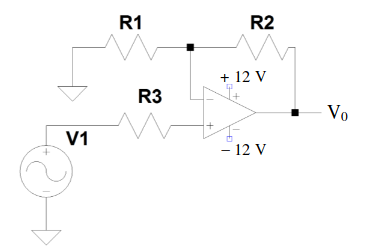
\includegraphics[scale = 0.5]{circuito.png}
  \caption{Circuito amplificador não-inversor com compensação para efeito da corrente de polarização.}
  \label{fig:circuito}
\end{figure}

Para este experimento, a mesma montagem foi realizada uma vez para cada um dos seguintes valores de $R_1$ e $R_2$ (medidos):
\begin{itemize}
  \item Montagem 1 - $R_1 = 197,8k\Omega$ e $R_2 = 202,3k\Omega$
  \item Montagem 2 - $R_1 = 98,9k\Omega$ e $R_2 = 98,3k\Omega$
  \item Montagem 3 - $R_1 = 99,9\Omega$ e $R_2 = 99,0\Omega$
\end{itemize}

\subsubsection{Parte 1 - Montagem}

O circuito da figura \ref{fig:circuito1} foi montado, obtendo-se a montagem da figura \ref{fig:montagem1}.

\begin{figure}[h]
  \centering
  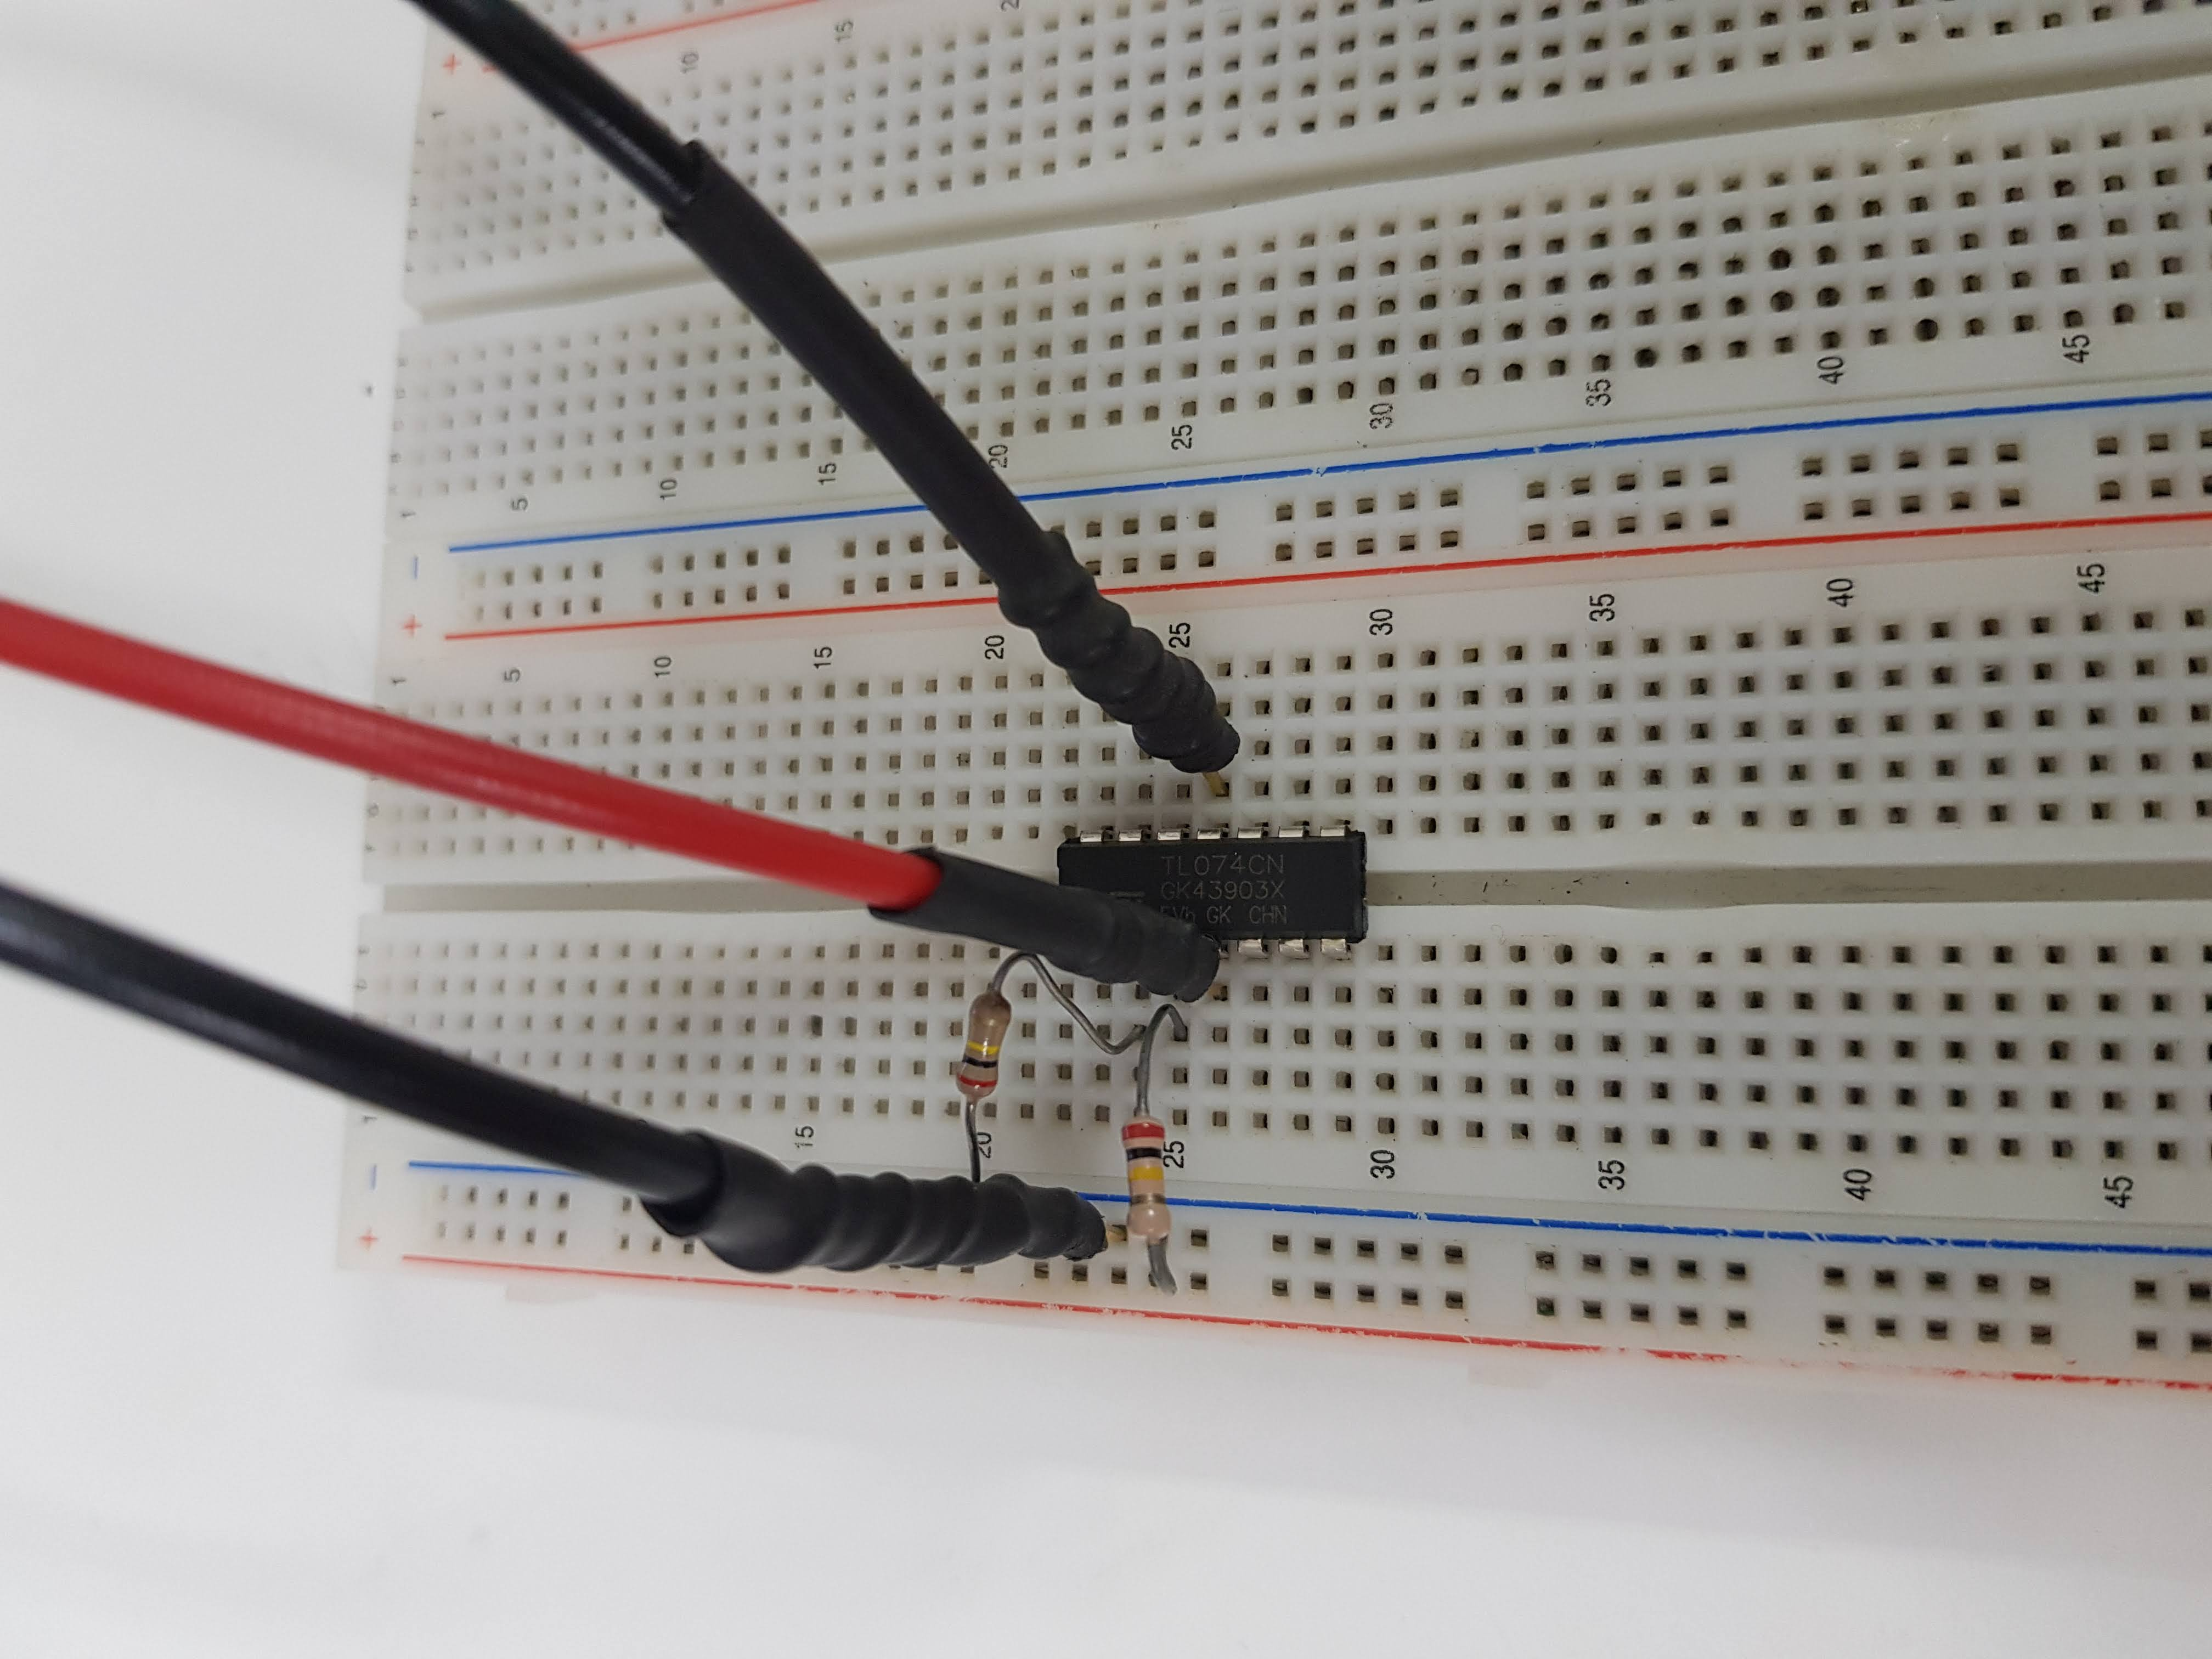
\includegraphics[width = 0.7\textwidth]{circ_0.jpg}
  \caption{Montagem do circuito da figura \ref{fig:circuito1}.}
  \label{fig:montagem1}
\end{figure}

\subsubsection{Parte 2}

  Foi medida a tensão DC nos terminais inversor e não-inversor, obtendo os seguintes valores para cada montagem:
  \begin{itemize}
    \item Montagem 1 - $V- = 1,7mV$ e $V+ = 1,7mV$
    \item Montagem 2 - $V- = 0,8mV$ e $V+ = 0,8mV$
    \item Montagem 3 - $V- = 0V$ e $V+ = 0V$
  \end{itemize}

\subsubsection{Parte 3}

  Utilizando a lei de Ohm e a fórmula fornecida no roteiro (\ref{eq:eq1}), foi calculada a corrente de compensação de entrada para cada montagem:
\begin{equation}
    $I_B = (I_B⁺ + I_B⁻)/2 $
  \label{eq:eq1}
\end{equation}

\begin{itemize}
  \item Montagem 1 - $I_B⁺ = 8,4nA$, $I_B⁻ = 8,59nA$ e $I_B = 8,5nA$
  \item Montagem 2 - $I_B⁺ = 8,14nA$, $I_B⁻ = 8,09nA$ e $I_B = 8,11nA$
  \item Montagem 3 - $I_B⁺ = 0A$, $I_B⁻ = 0A$ e $I_B = 0A$
\end{itemize}

\subsubsection{Parte 4}
  Foi calculada a a diferença entre correntes de compensação para a determinação da corrente de polarização para cada montagem:
  \begin{itemize}
    \item Montagem 1 - $I_O_S = -0,19nA$
    \item Montagem 2 - $I_O_S = 0,05nA$
    \item Montagem 3 - $I_O_S = 0A$
  \end{itemize}
\pagebreak
\subsubsection{Parte 5}

Após a aquisição de todos os dados necessários, foi construída a seguinte tabela:

\begin{table}[h!]
\centering
\begin{tabular}[width = 0.8\textwidth]{|l|l|l|l|}
  \hline
  Frequência (Hz) & Amplitude $V_1$ (V) & Amplitude $V_O$ & R2_{medido} & V^- (mV) & V^+ (mV) & I_B^- (nA) & I_B^+ (nA) & I_B (nA) & I_{OS} (nA) \\
  \hline
  200k\Omega & 200k\Omega & 197,8k\Omega & 202,3k\Omega & 1,7 & 1,7 & 8,59 & 8,4 & 8,5 & 0 \\
  \hline
  100k\Omega & 100k\Omega & 98,9k\Omega & 98,3k\Omega & 0,8 & 0,8 & 8,09 & 8,14 & 8,11 & 0 \\
  \hline
  100\Omega & 100\Omega & 99,9\Omega & 99,0\Omega & 0 & 0 & 0 & 0 & 0 & 0 \\
  \hline
\end{tabular}
\caption{Correntes de compensação (bias) e de polarização (offset) de entrada}
\label{tab:exp1}
\end{table}

%\clearpage

\subsection{Experiência 2}

Foi montado o circuito de acordo com a figura \ref{fig:circuito2}, obtendo, assim, a montagem da figura \ref{fig:montagem2}.

\begin{figure}[h]
  \centering
  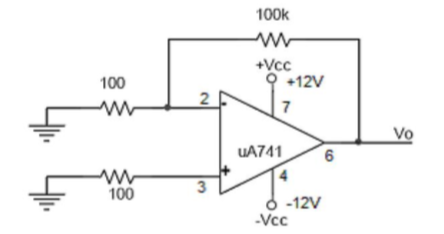
\includegraphics[scale = 0.5]{exp2.png}
  \caption{Circuito para medida das tensões de compensação de entrada e saída.}
  \label{fig:circuito2}
\end{figure}

Para este experimento, a mesma montagem foi realizada uma vez para cada um dos seguintes valores de R (medidos):
\begin{itemize}
  \item Montagem 1 - $R = 98,9k\Omega$
  \item Montagem 2 - $R = 202,3k\Omega$
  \item Montagem 3 - $R = 978\Omega$
\end{itemize}

\subsubsection{Parte 1 - Montagem}

O circuito da figura \ref{fig:circuito2} foi montado, obtendo-se a montagem da figura \ref{fig:montagem2}.

\begin{figure}[h]
  \centering
  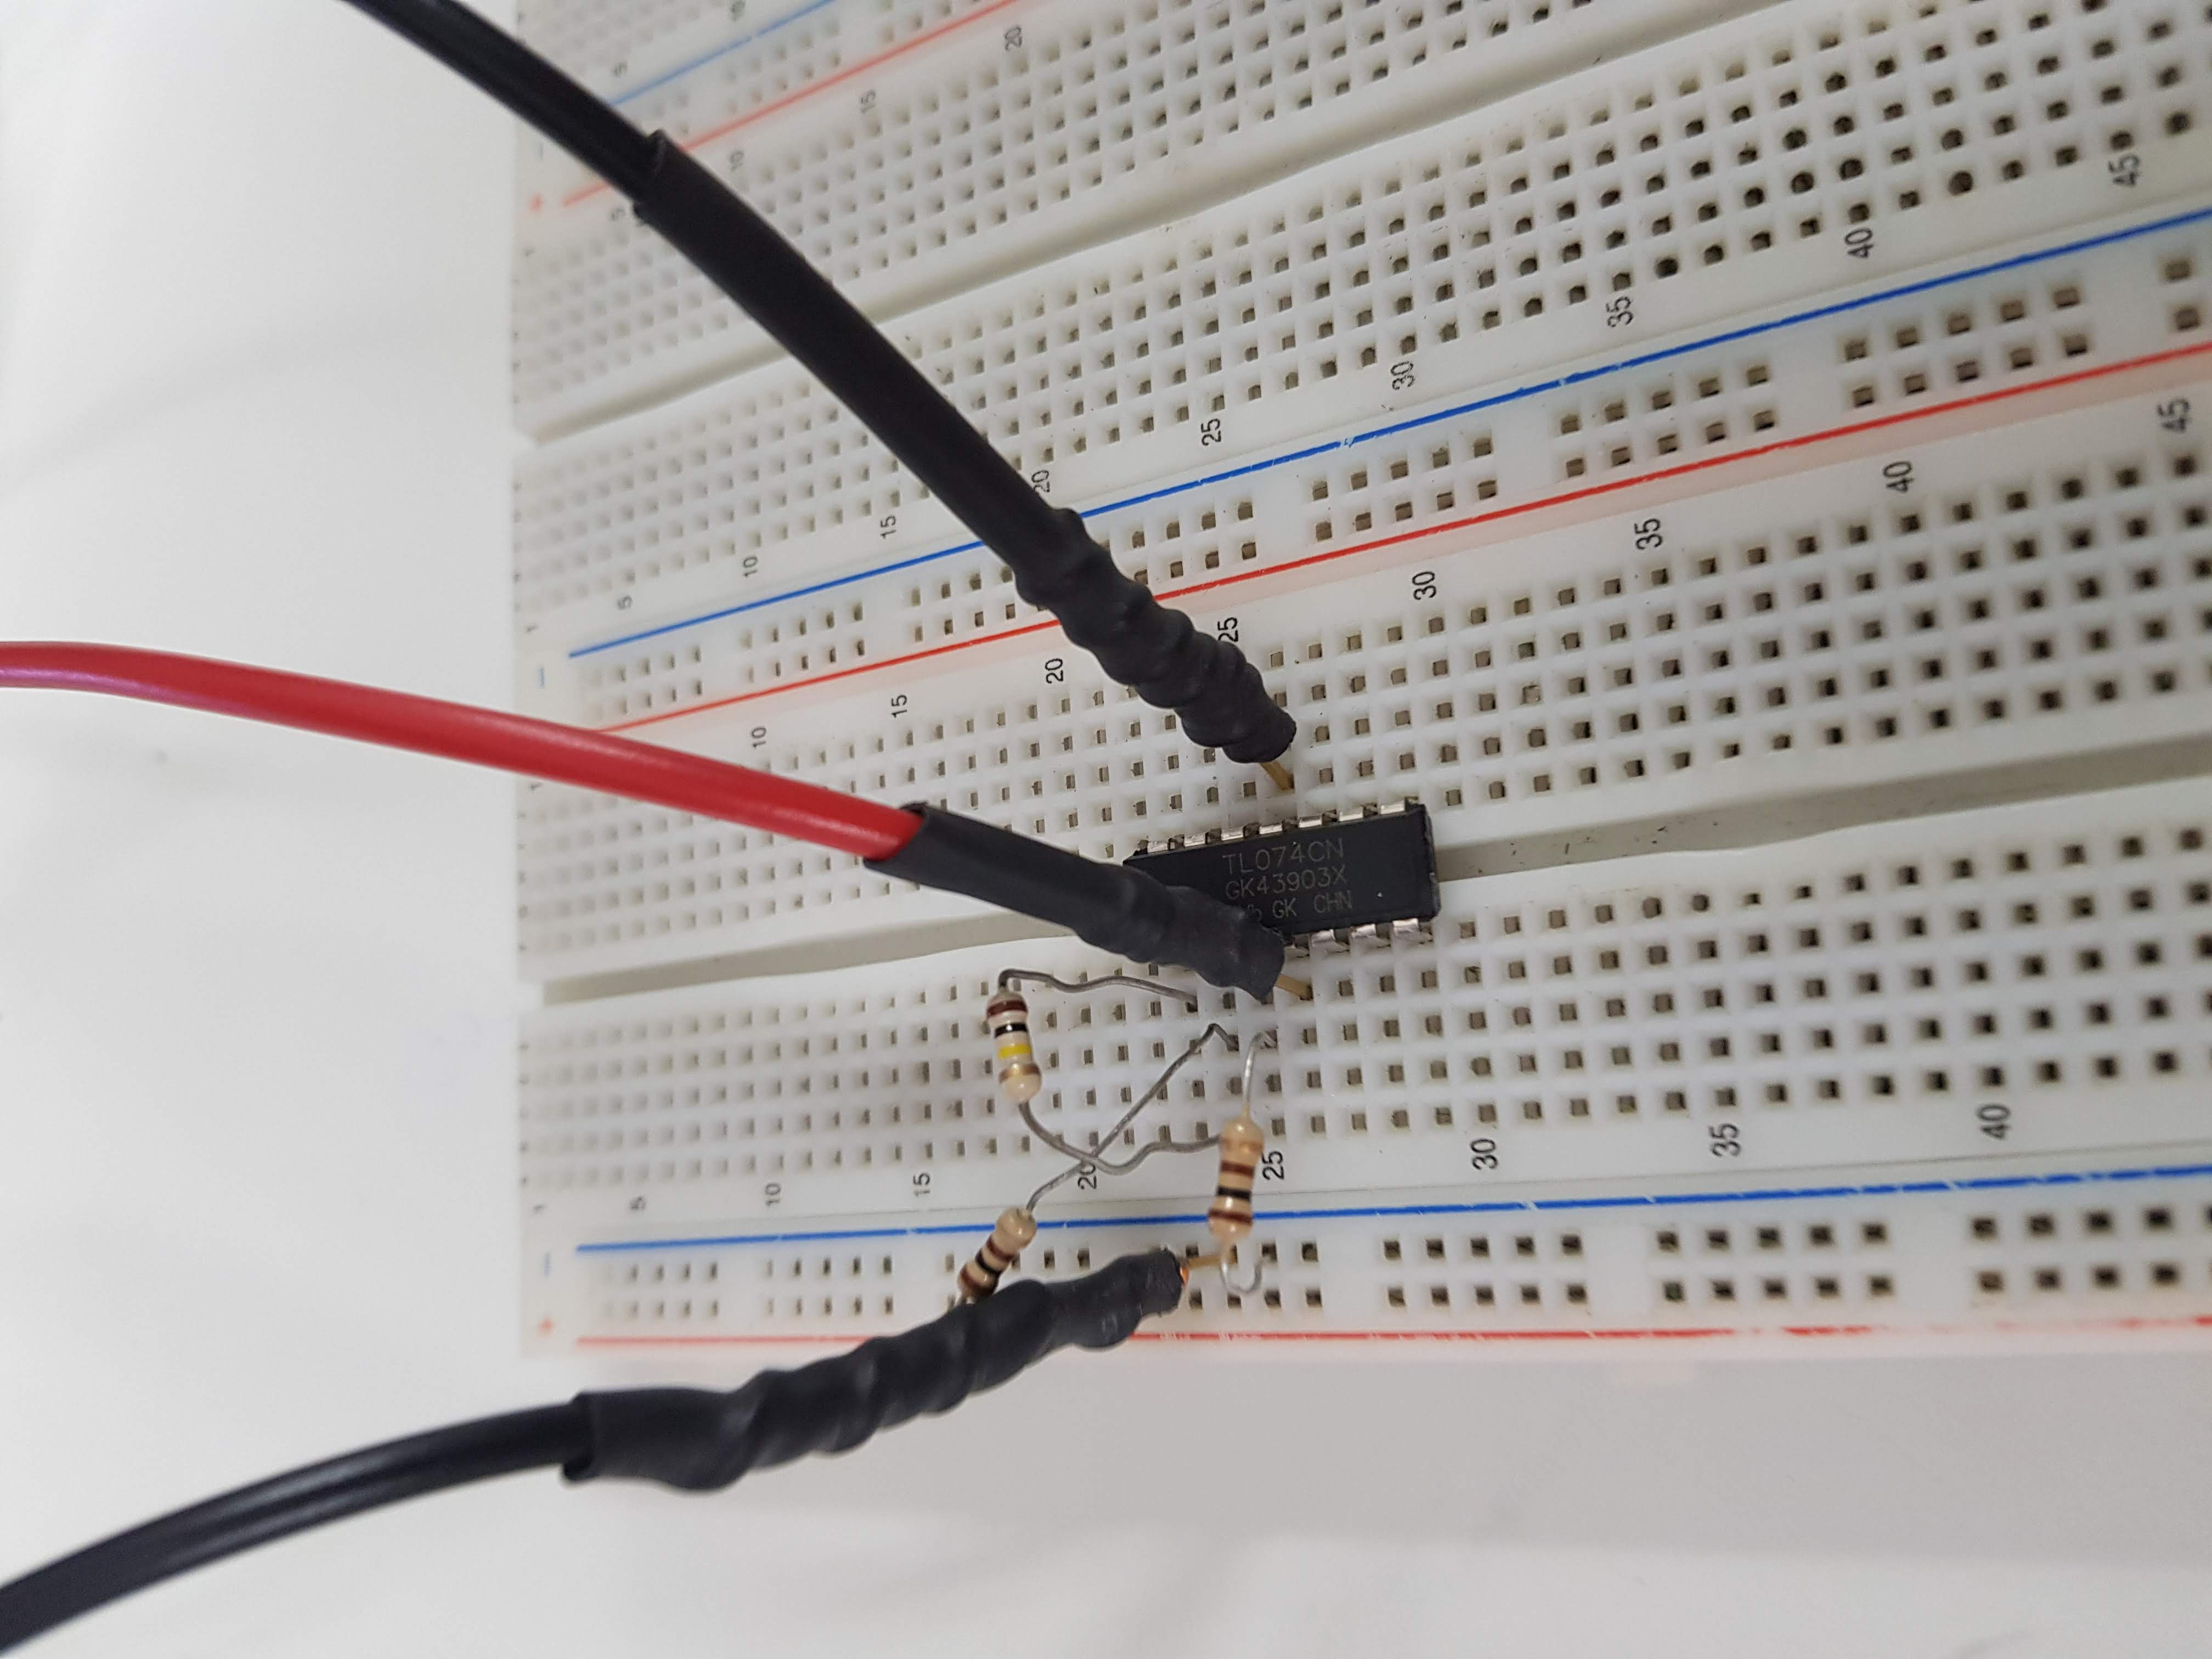
\includegraphics[width = 0.7\textwidth]{circ_1.jpg}
  \caption{Montagem do circuito da figura \ref{fig:circuito2}.}
  \label{fig:montagem2}
\end{figure}

\subsubsection{Parte 2}
Para cada montagem, foi medida a tensão DC de saída:
\begin{itemize}
  \item Montagem 1 - $V_o = -0,47V$
  \item Montagem 2 - $V_o = -0,95V$
  \item Montagem 3 - $V_o = -5,1mV$
\end{itemize}
\subsubsection{Parte 3}
Para cada montagem foi calculada a tensão de polarização de entrada:

\begin{itemize}
  \item Montagem 1 - $V_o_s = -0,47mV$
  \item Montagem 2 - $V_o_s = -0,47mV$
  \item Montagem 3 - $V_o_s = -0,47mV$
\end{itemize}

\subsubsection{Parte 4}
Após a aquisição dos dados necessários, foi construída a seguinte tabela:

\begin{table}[h!]
\centering
\begin{tabular}{|l|l|l|l|}
  \hline
   & Resistor & Tensão DC de saída (V) & Tensão de offset de entrada (mV) \\
  \hline
  \multirow{3}{8em}{Primeiro CI LM741} & 100k\Omega & -0,47 & -0.47 \\
   & 200k\Omega & -0,95 & -0.47 \\
   & 1k\Omega & -0,0051 & -0.47 \\
  \hline
\end{tabular}
\caption{Tensões offset de entrada e saída para o amplificador operacional LM741}
\label{tab:exp2}
\end{table}

\clearpage

\subsection{Experiência 3}

Foram montados os circuitos de acordo com a figura \ref{fig:circuito3}, obtendo, assim, as montagens das figuras \ref{fig:montagem3} e \ref{fig:montagem4}.

\begin{figure}[h]
  \centering
  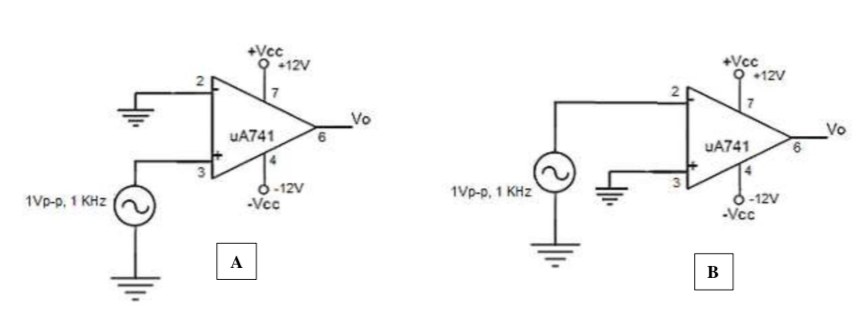
\includegraphics[scale = 0.5]{exp3.png}
  \caption{circuitos para medição das tensões de saturação.}
  \label{fig:circuito3}
\end{figure}

\subsubsection{Parte 1 - Montagem}

Os circuitos da figura \ref{fig:circuito3} foram montados, obtendo-se as montagens das figuras \ref{fig:montagem3} e \ref{fig:montagem4}.

\begin{figure}[h]
  \centering
  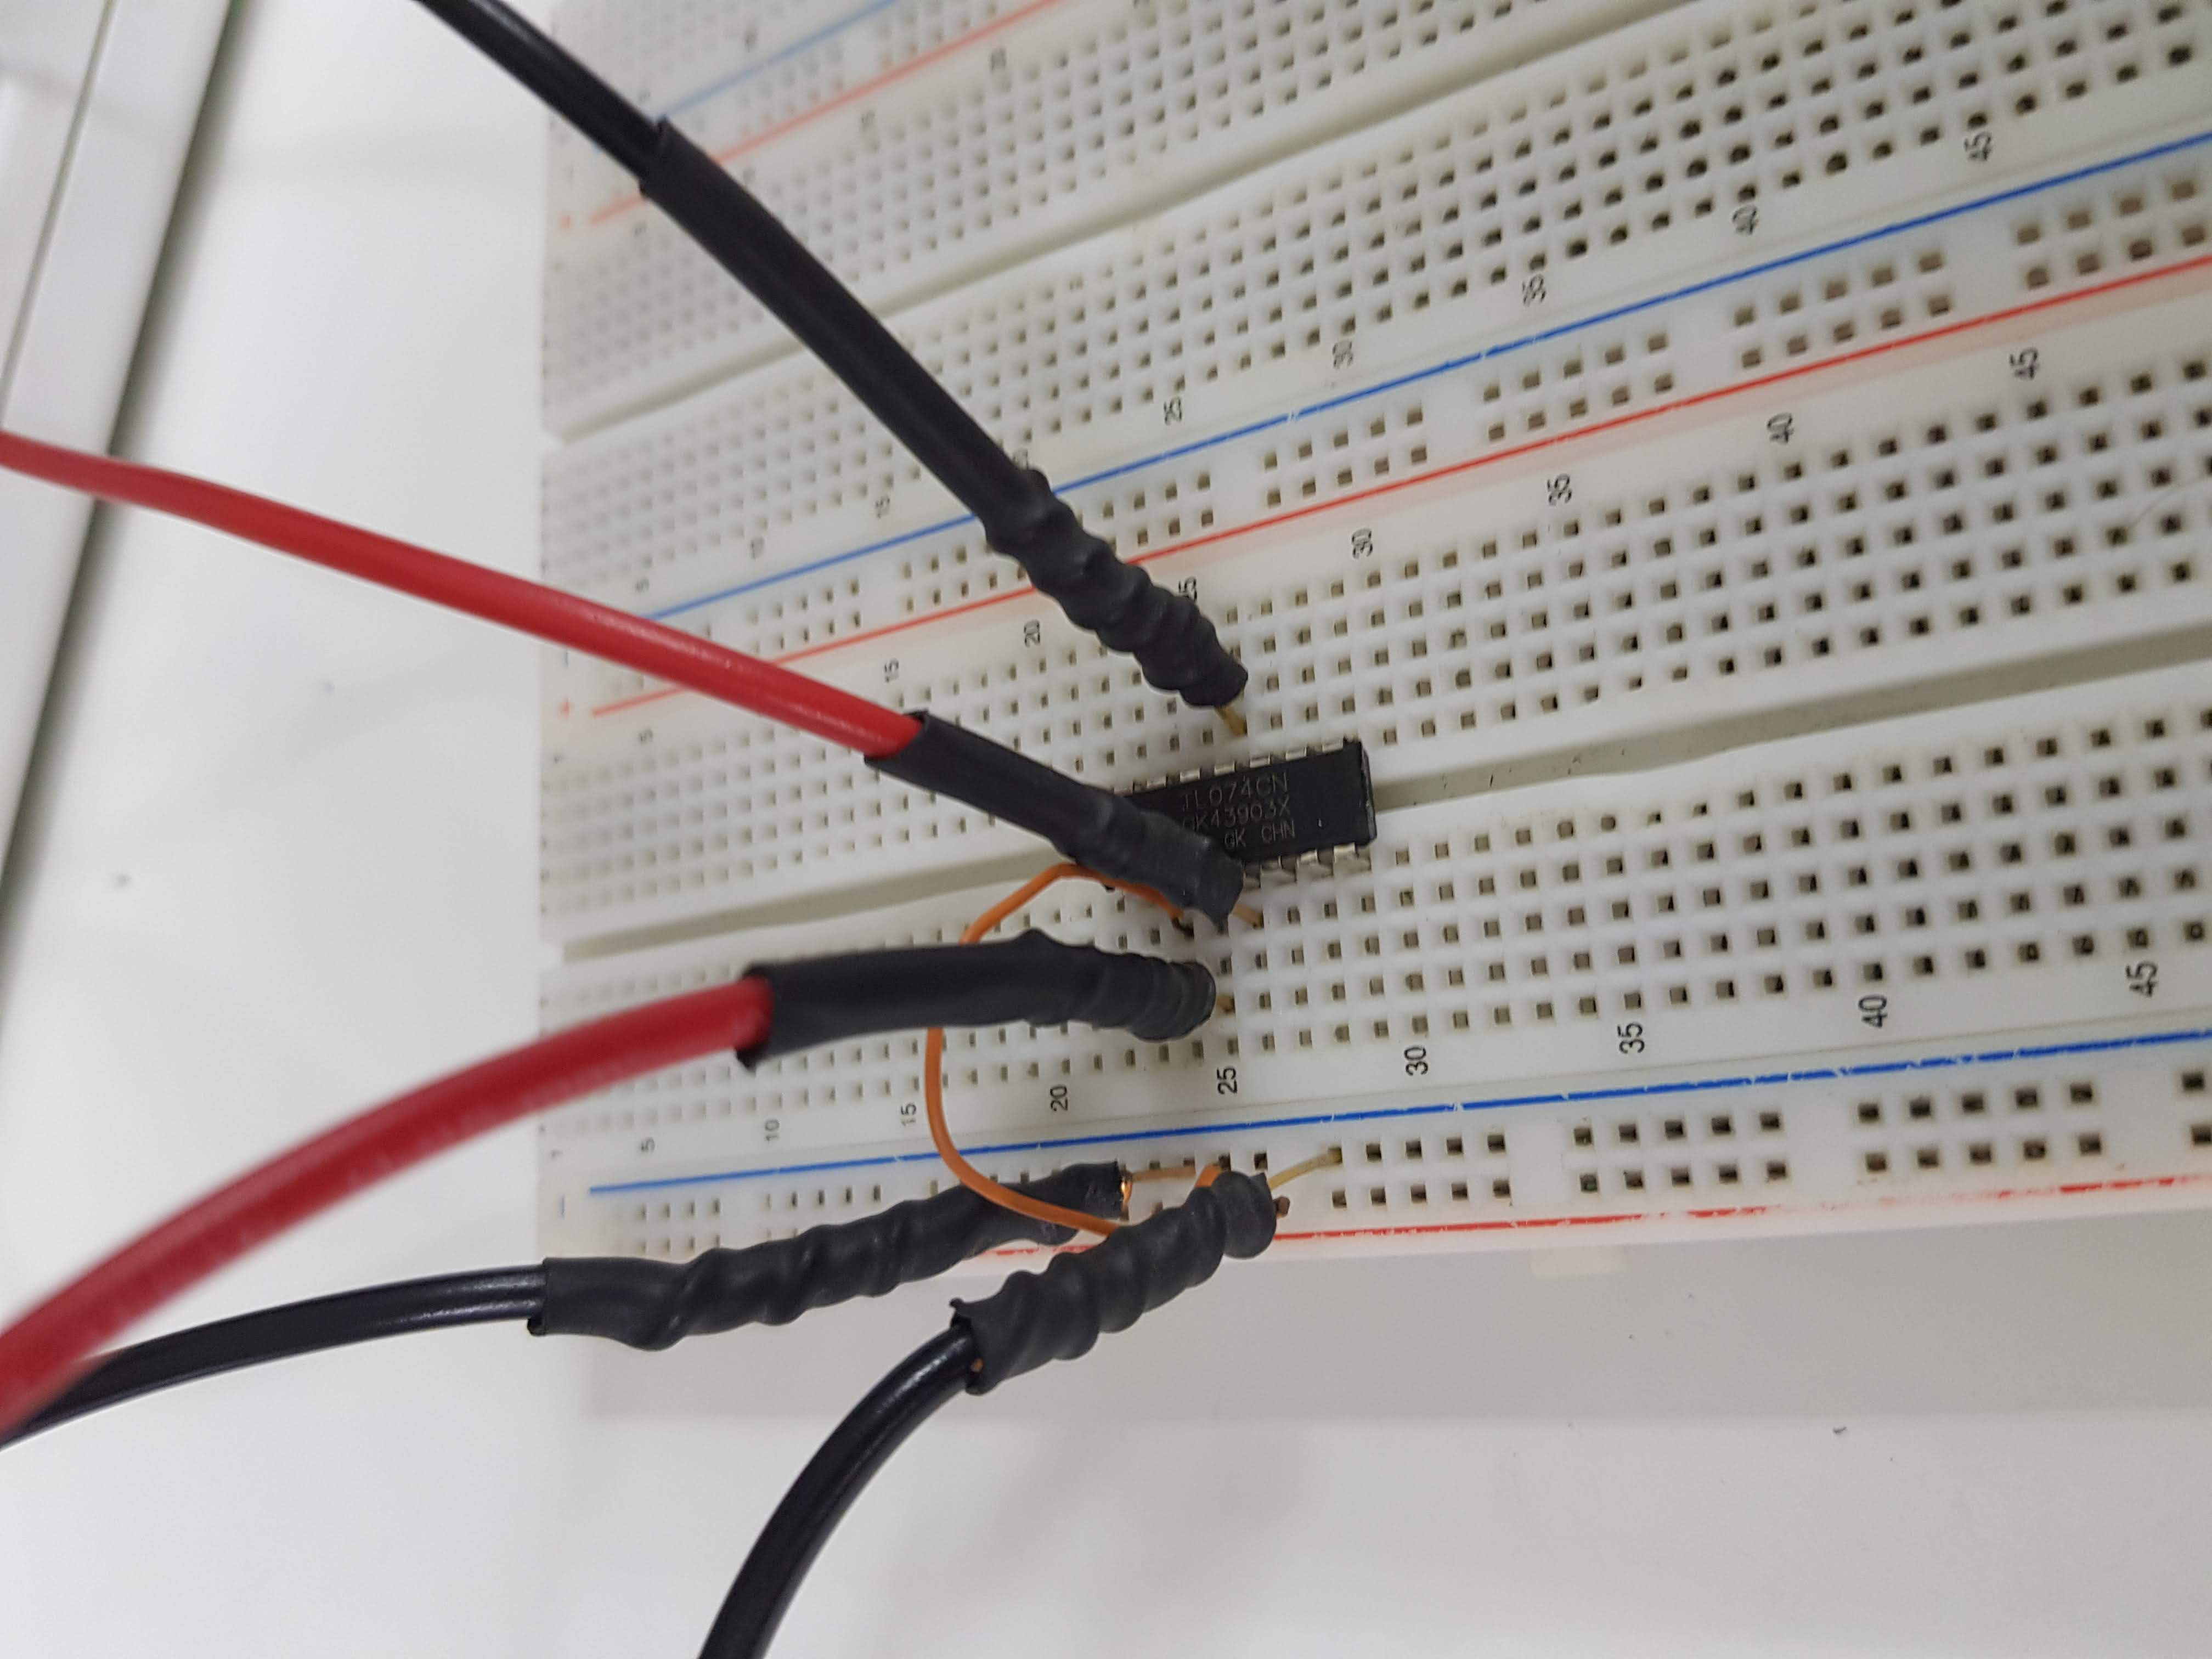
\includegraphics[width = 0.7\textwidth]{circ_2.jpg}
  \caption{Montagem do circuito da figura \ref{fig:circuito3} A.}
  \label{fig:montagem3}
\end{figure}
\begin{figure}[h]
  \centering
  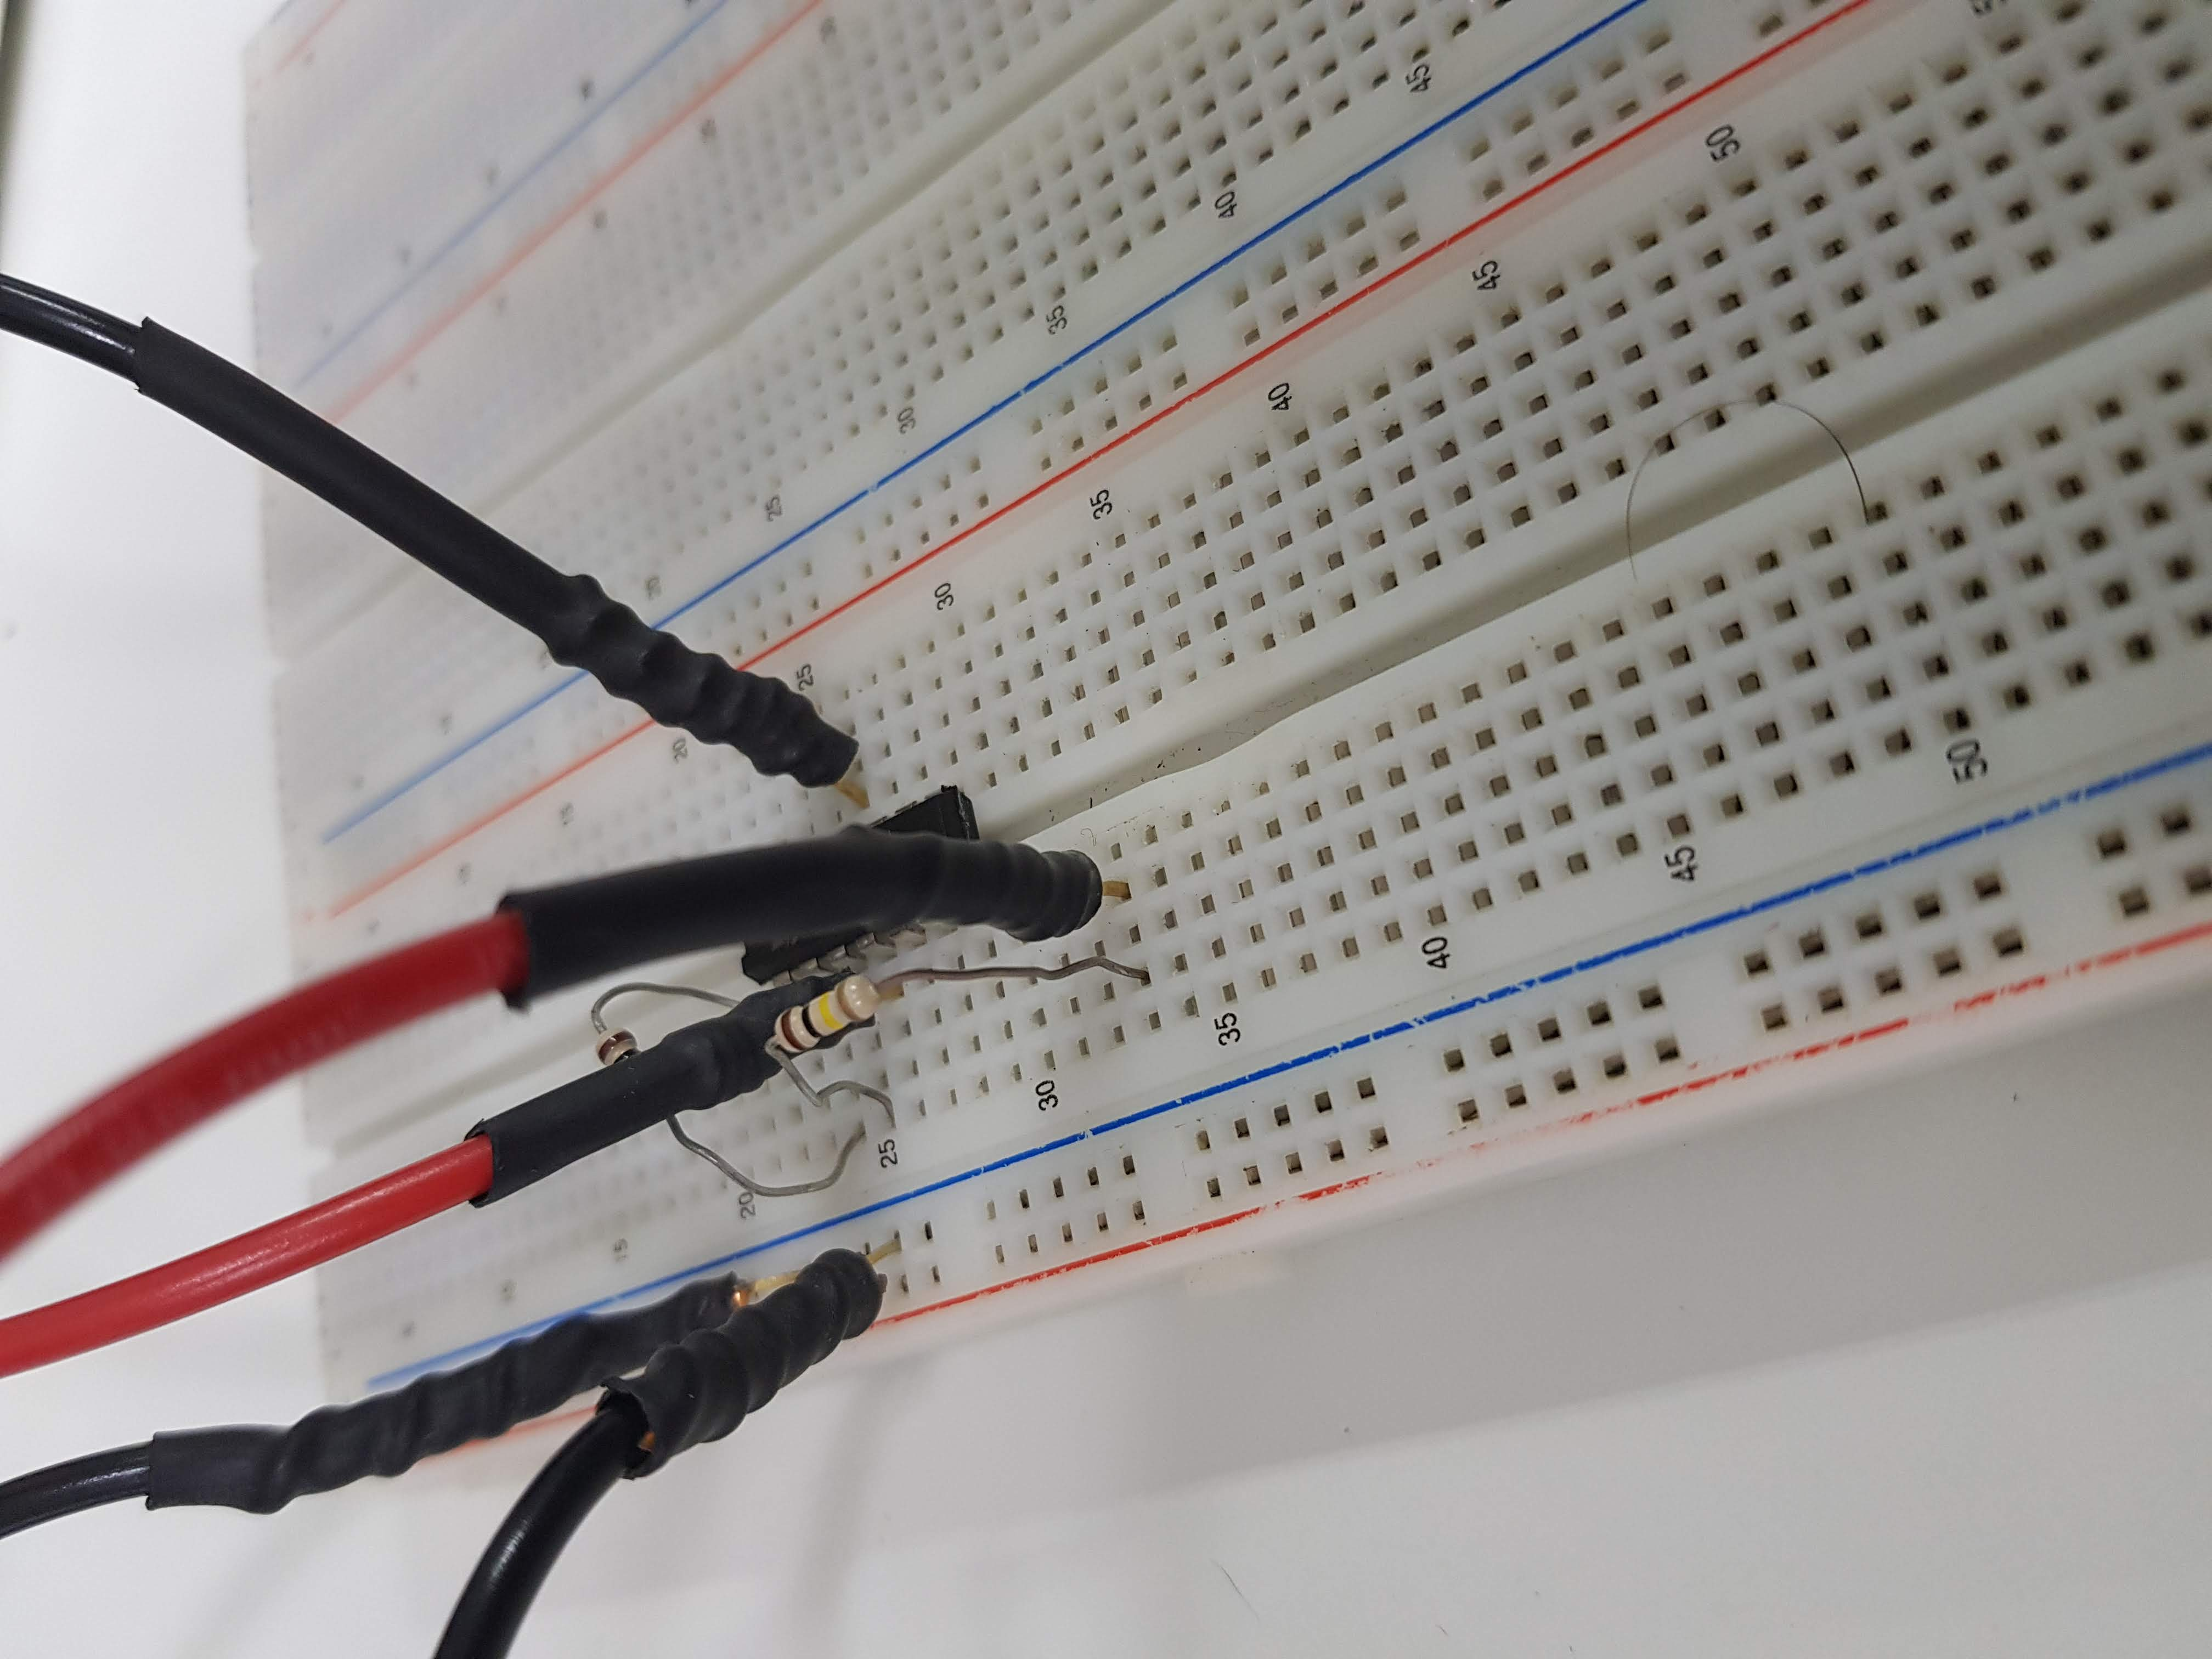
\includegraphics[width = 0.7\textwidth]{circ_3.jpg}
  \caption{Montagem do circuito da figura \ref{fig:circuito3} B.}
  \label{fig:montagem4}
\end{figure}

\subsubsection{Parte 2}
Para cada montagem, foram visualizadas no osciloscópio as ondas de entrada e saída, obtendo as imagens \ref{fig:inout1} e \ref{fig:inout2} para as montagens.
\begin{figure}[h]
  \centering
  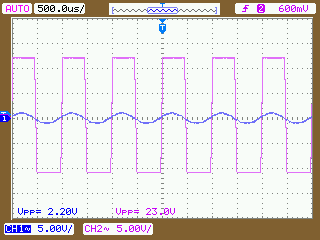
\includegraphics[scale = 0.5]{NewFile0.png}
  \caption{Ondas de entrada e saída para o circuito da figura \ref{fig:circuito3} A.}
  \label{fig:inout1}
\end{figure}
\begin{figure}[h]
  \centering
  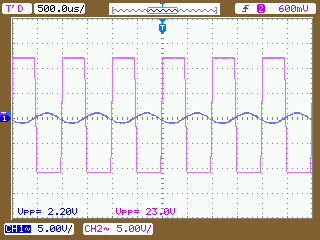
\includegraphics[scale = 0.5]{NewFile1.png}
  \caption{Ondas de entrada e saída para o circuito da figura \ref{fig:circuito3} B.}
  \label{fig:inout2}
\end{figure}
\pagebreak
\subsubsection{Parte 3}

Após a aquisição dos dados necessários, foi construída a seguinte tabela:

\begin{table}[h!]
\centering
\begin{tabular}{|l|l|l|}
  \hline
   & Tensão AC pico-a-pico de entrada (V) & Tensão AC pico-a-pico de saída (V) \\
  \hline
  Figura \ref{fig:circuito3} A & 2,2 & 23 \\
  \hline
  Figura \ref{fig:circuito3} B & 2,2 & 23 \\
  \hline
\end{tabular}
\caption{Tensões de saturação}
\label{tab:exp3}
\end{table}

%\clearpage

\subsection{Experiência 4}

Foram montados os circuitos de acordo com as figuras \ref{fig:circuito4} e \ref{fig:circuito5}, obtendo, assim, as montagens das figuras \ref{fig:montagem5} e \ref{fig:montagem6}.
Para ambas as montagens, $R_i_n = 98,3k\Omega e R_o_u_t = 98,9k\Omega$.
\begin{figure}[h]
  \centering
  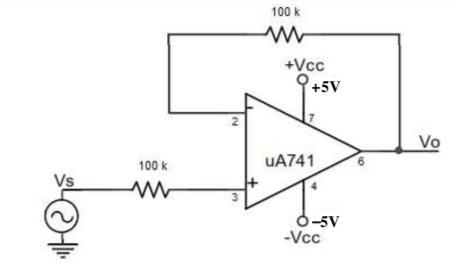
\includegraphics[scale = 0.5]{exp4-1.png}
  \caption{Medição da faixa de tensão de entrada.}
  \label{fig:circuito4}
\end{figure}
\begin{figure}[h]
  \centering
  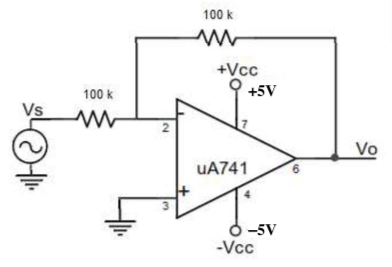
\includegraphics[scale = 0.5]{exp4-2.png}
  \caption{Medição dos intervalos de tensão de saída.}
  \label{fig:circuito5}
\end{figure}

\subsubsection{Parte 1 - Montagem}

Os circuitos das figuras \ref{fig:circuito4} e \ref{fig:circuito5} foram montados, obtendo-se as montagens das figuras \ref{fig:montagem5} e \ref{fig:montagem6}, respectivamente.

\begin{figure}[h]
  \centering
  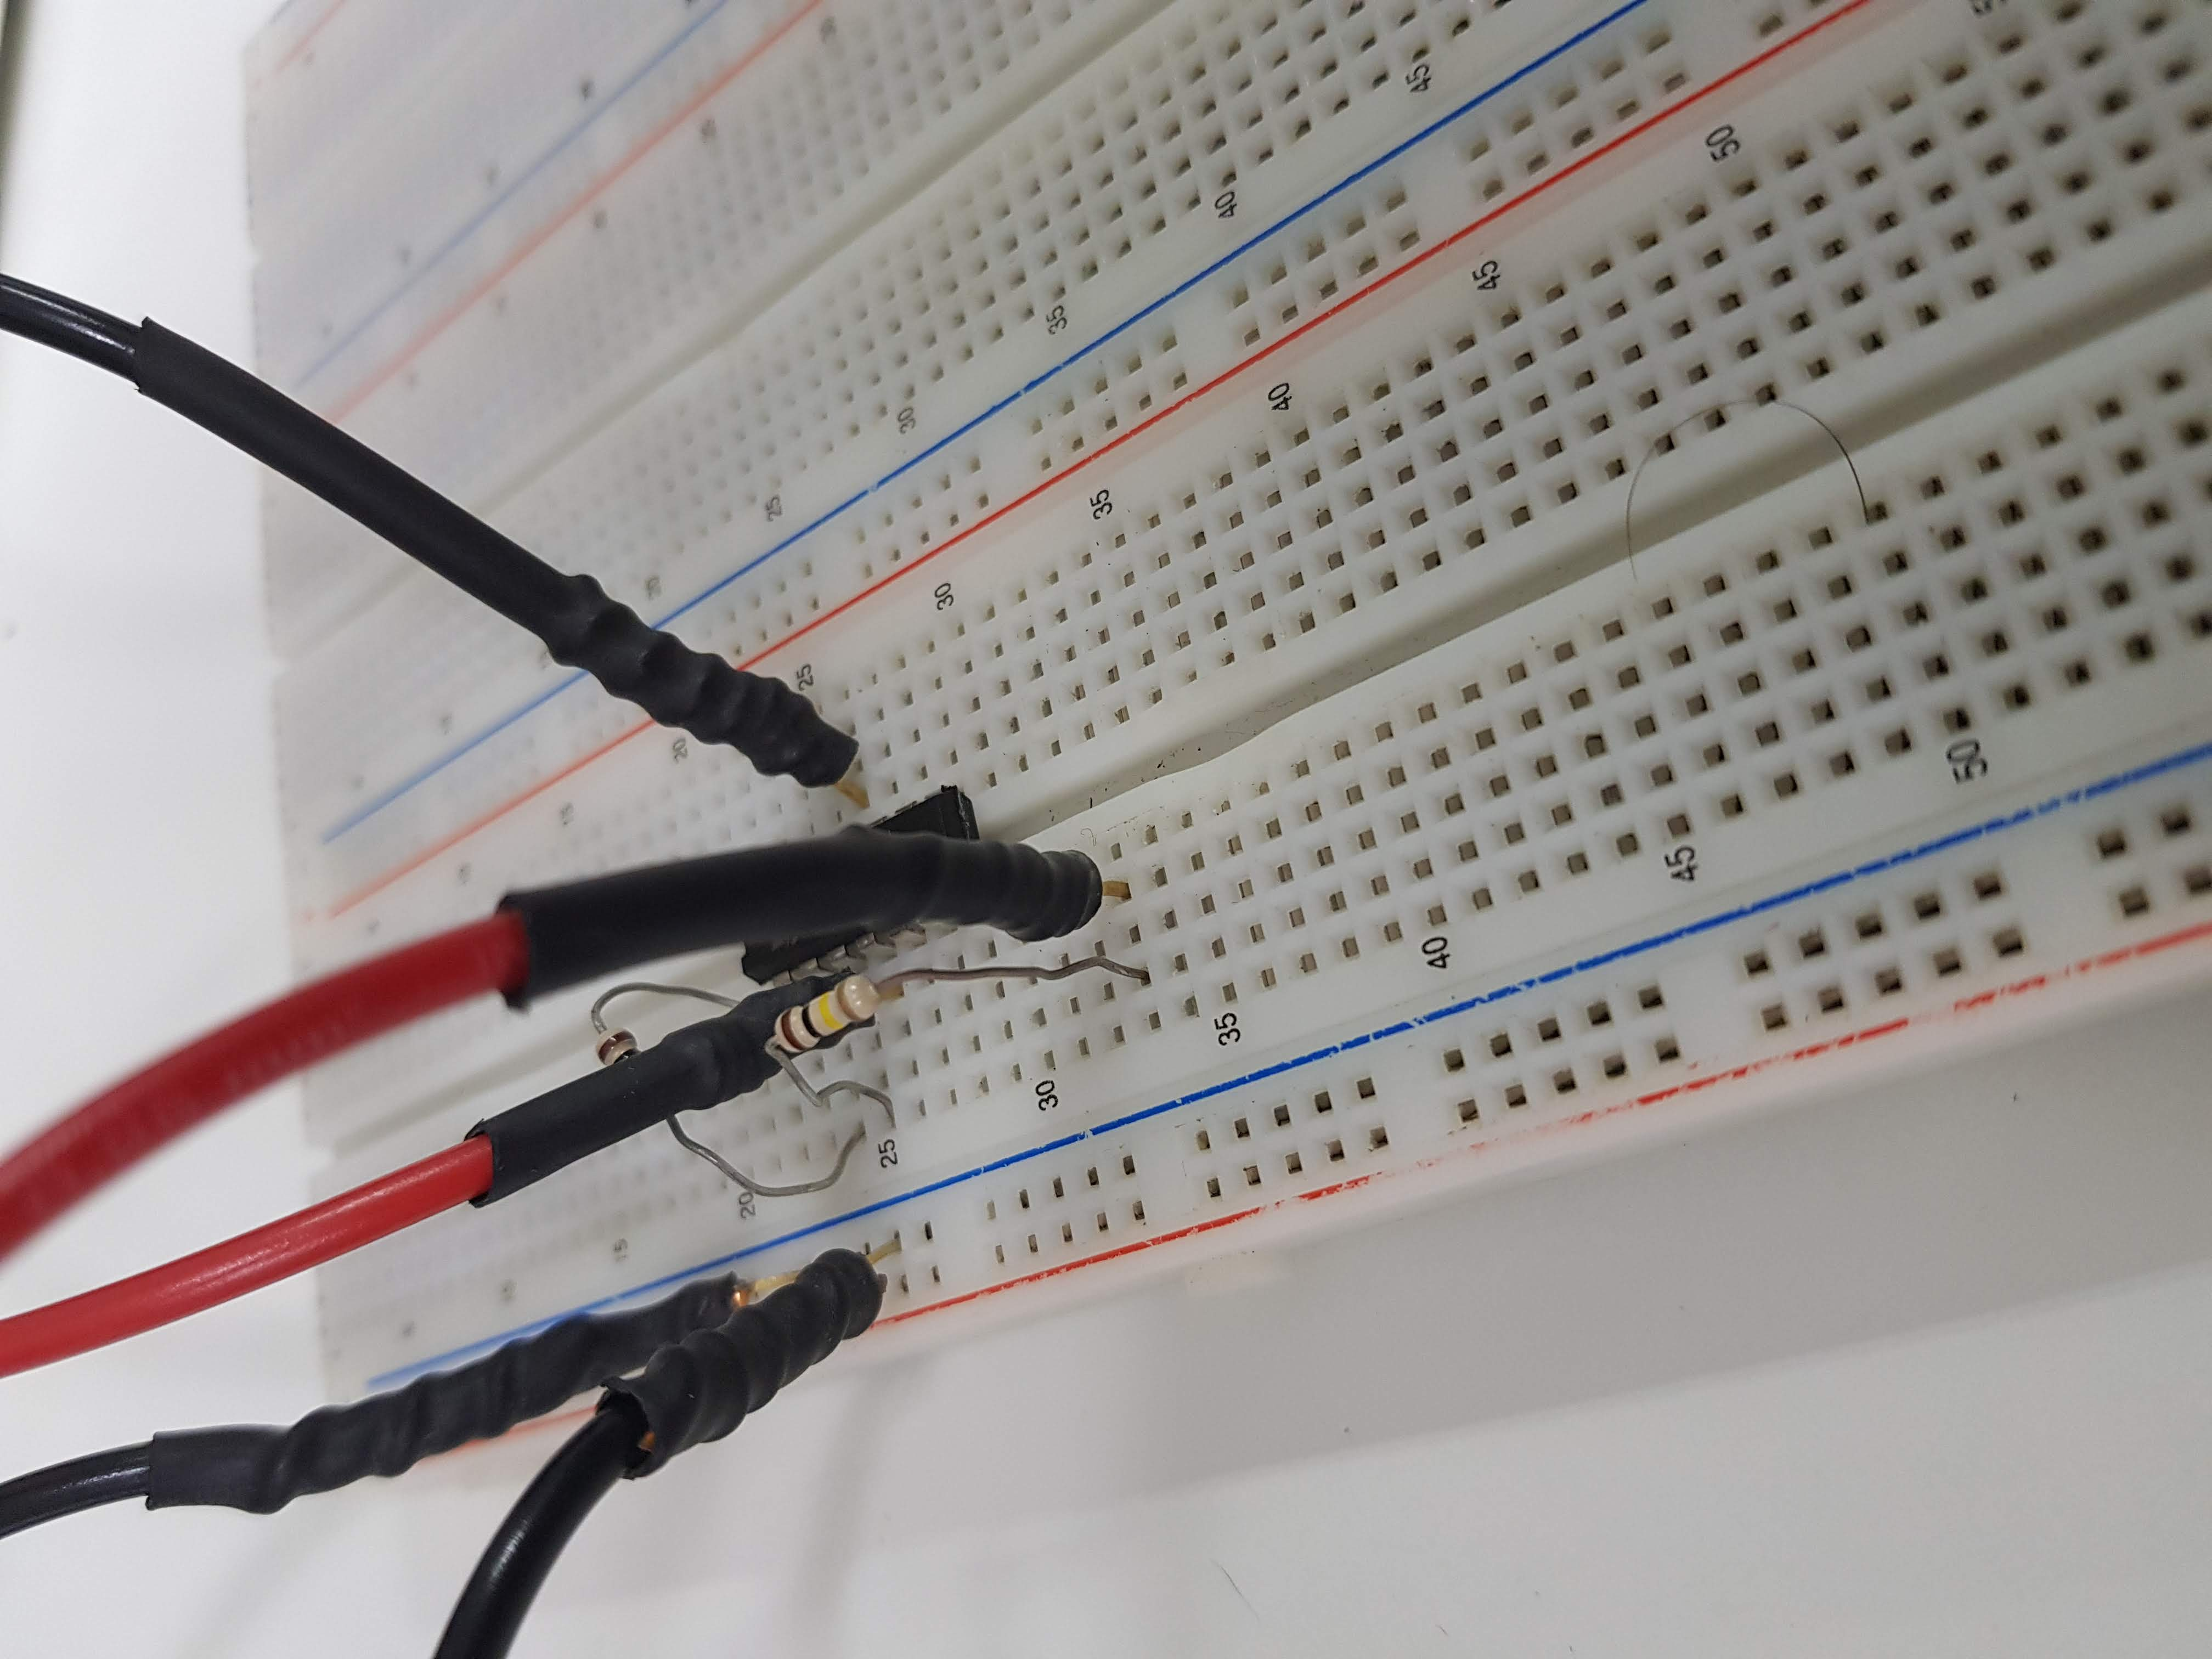
\includegraphics[width = 0.7\textwidth]{circ_3.jpg}
  \caption{Montagem do circuito da figura \ref{fig:circuito4}.}
  \label{fig:montagem5}
\end{figure}
\begin{figure}[h]
  \centering
  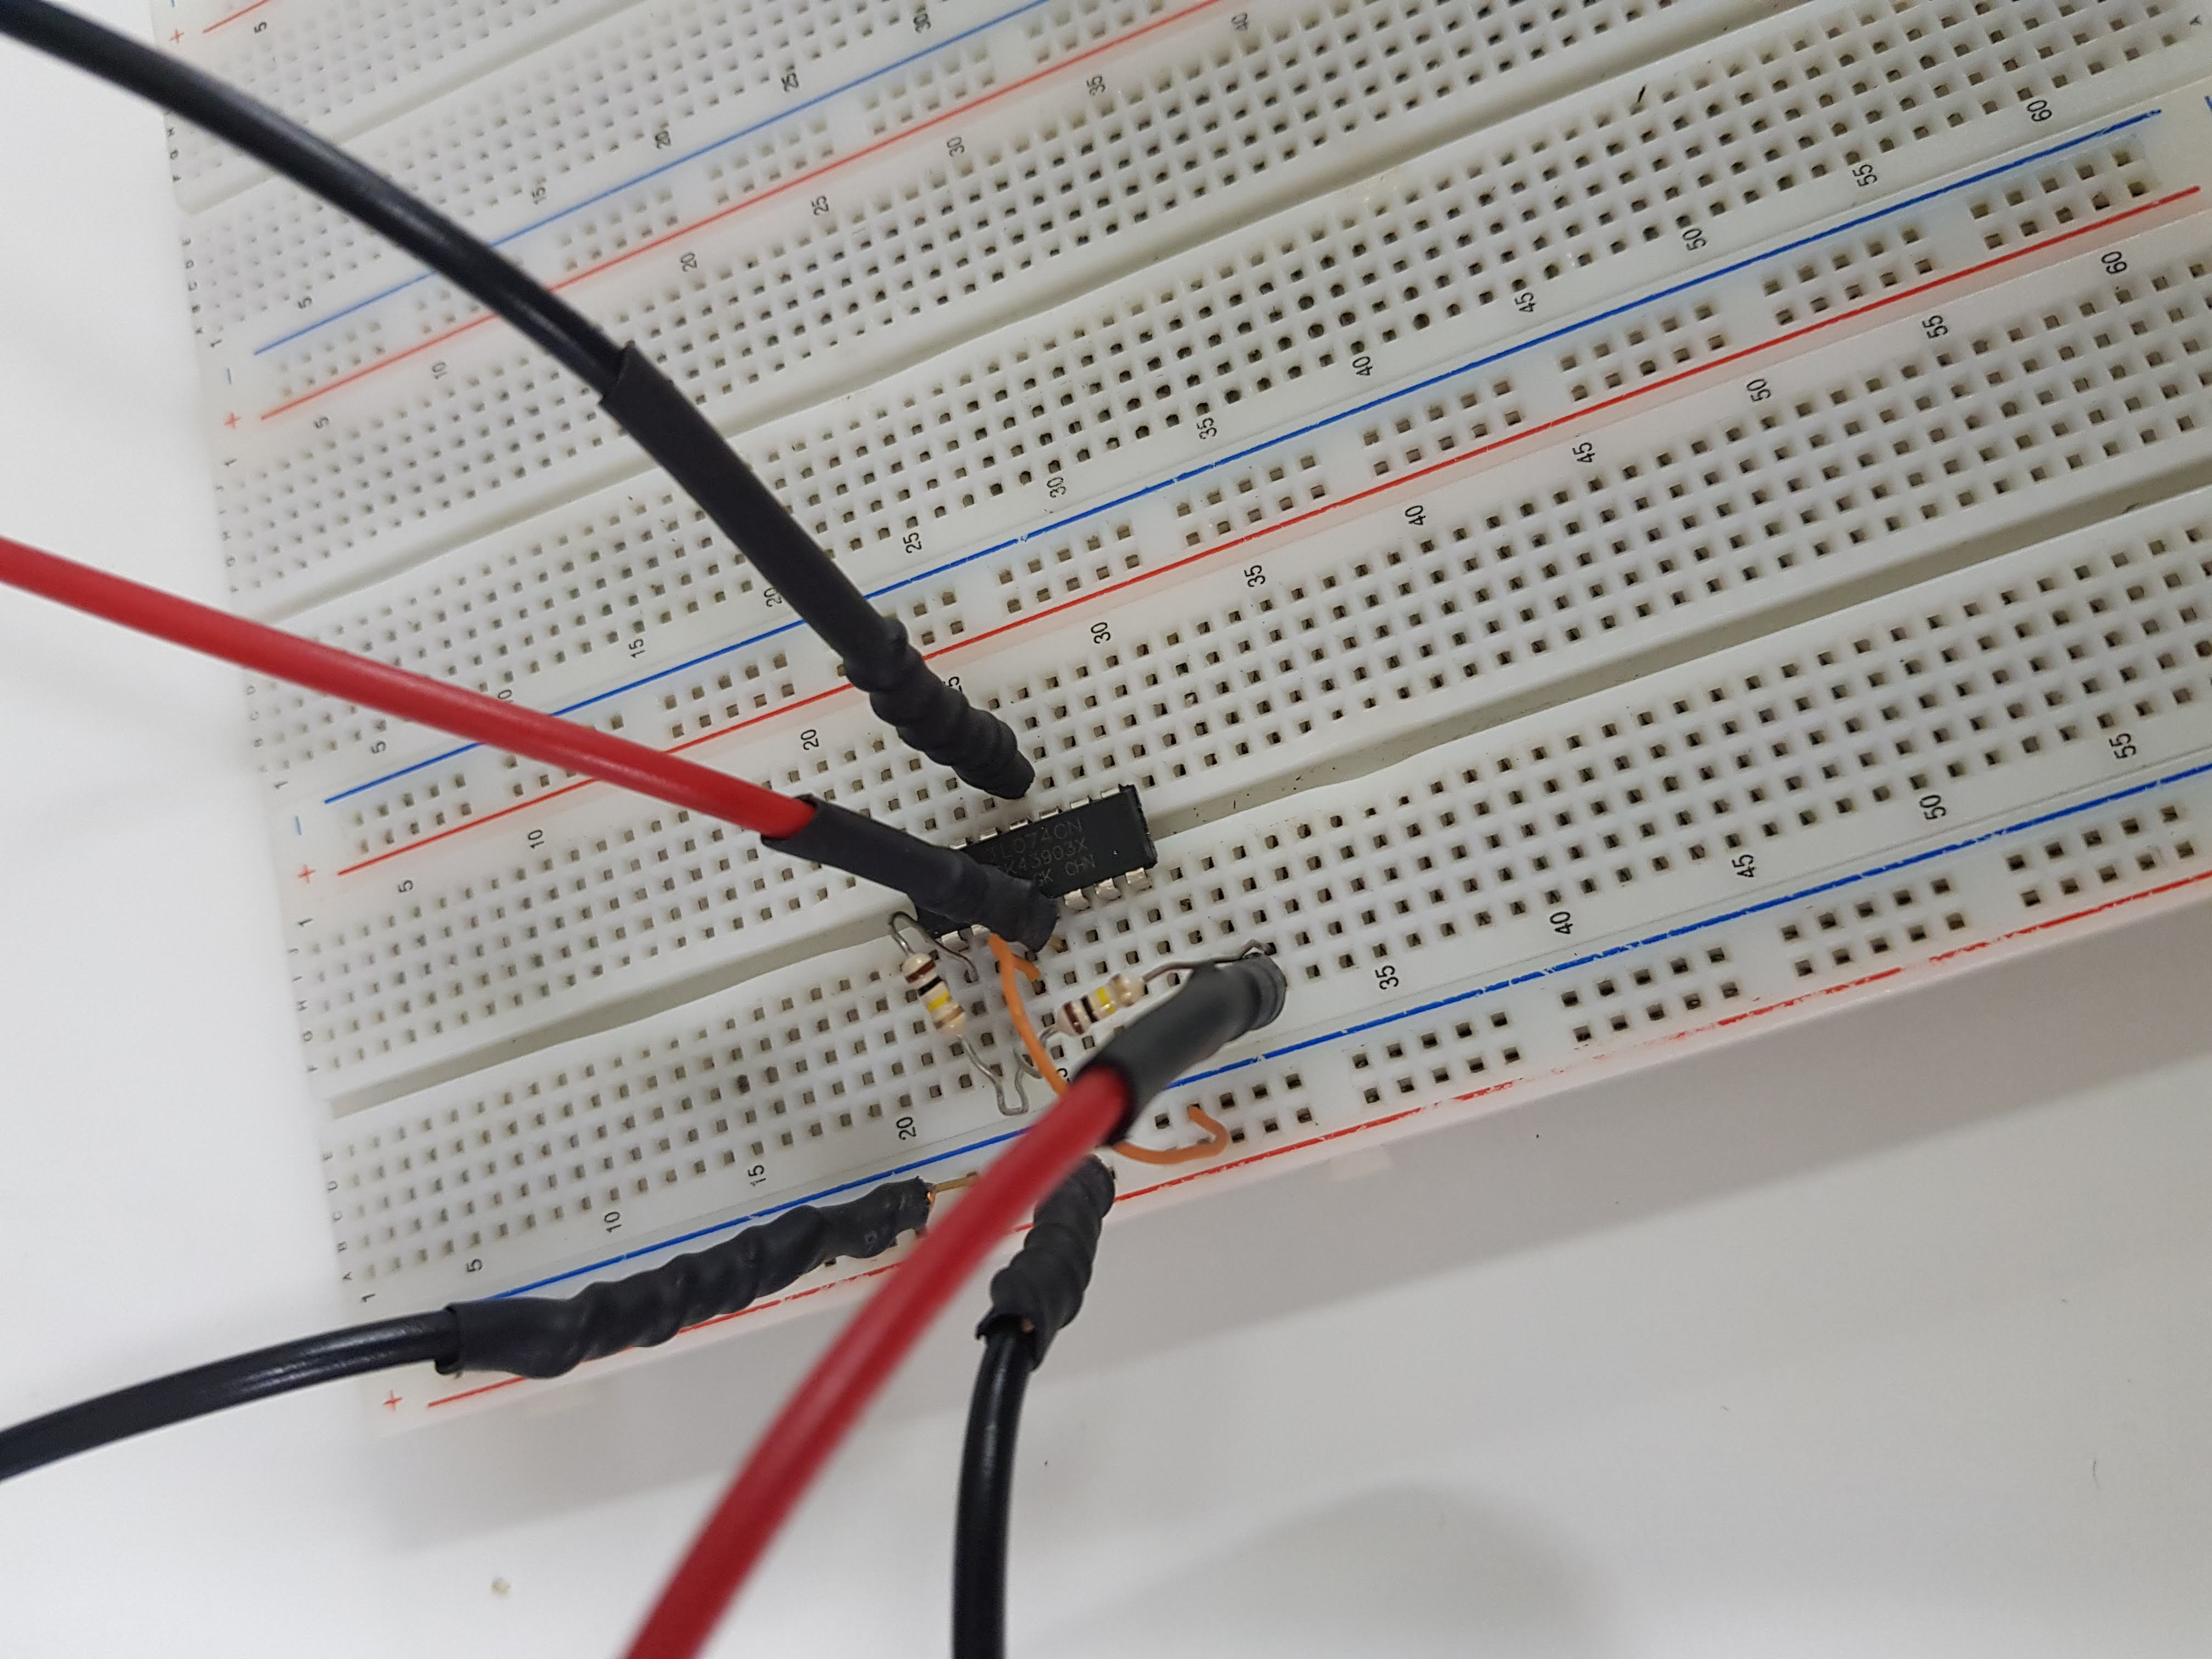
\includegraphics[width = 0.7\textwidth]{circ_4.jpg}
  \caption{Montagem do circuito da figura \ref{fig:circuito5}.}
  \label{fig:montagem6}
\end{figure}

\subsubsection{Parte 2}
Para a montagem da figura \ref{fig:montagem5}, foi visualizada no osciloscópio as ondas de entrada e saída, utilizando uma entrada senoidal de 5V de amplitude e 100Hz de frequência obtendo a imagen \ref{fig:inout3}.
\begin{figure}[h]
  \centering
  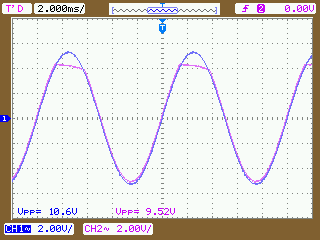
\includegraphics[scale = 0.5]{NewFile3.png}
  \caption{Ondas de entrada e saída para o circuito da figura \ref{fig:circuito4}.}
  \label{fig:inout3}
\end{figure}

\subsubsection{Parte 3}

Foi ajustada a fonte de tensão até que não fossem observadas distorções, obtendo o resultado da imagem \ref{fig:inout4}
\begin{figure}[h]
  \centering
  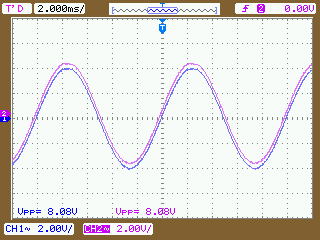
\includegraphics[scale = 0.5]{NewFile4.png}
  \caption{Ondas de entrada e saída para o circuito da figura \ref{fig:circuito4} com uma tensão de entrada que não exibe distorções na saída.}
  \label{fig:inout4}
\end{figure}

A amplitude de entrada colocada na fonte foi $3,9V$ e a tensão de pico a pico observada na saída foi $8,08V$. É possível observar que a tensão máxima em que não ocorrem distorções é controlada pelas tensões colocadas em $+/-V_{CC}$.

\subsubsection{Parte 4}
Foram medidos os valores de pico positivo e negativo da tensão de entrada, obtendo $8,08V$ na tensão de entrada, que é menor que as tensões colocadas em $+/-V_{CC}$, os valores máximos de pico a pico que podem ser colocados na entrada são limitados pelos valores em $+/-V_{CC}$.

\subsubsection{Parte 5}
Foi realizado o mesmo procedimento para o circuito \ref{fig:circuito5}.

Para a montagem da figura \ref{fig:montagem6}, foi visualizada no osciloscópio as ondas de entrada e saída, utilizando uma entrada senoidal de 5V de amplitude e 100Hz de frequência obtendo a imagen \ref{fig:inout5}.
\begin{figure}[h]
  \centering
  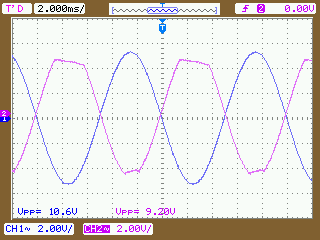
\includegraphics[scale = 0.5]{NewFile5.png}
  \caption{Ondas de entrada e saída para o circuito da figura \ref{fig:circuito5}.}
  \label{fig:inout5}
\end{figure}

Foi ajustada a fonte de tensão até que não fossem observadas distorções, obtendo o resultado da imagem \ref{fig:inout6}
\begin{figure}[h]
  \centering
  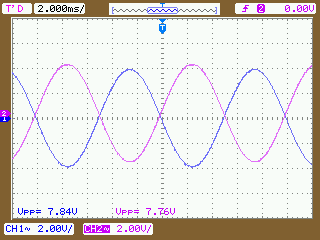
\includegraphics[scale = 0.5]{NewFile6.png}
  \caption{Ondas de entrada e saída para o circuito da figura \ref{fig:circuito5} com uma tensão de entrada que não exibe distorções na saída.}
  \label{fig:inout6}
\end{figure}

A amplitude de entrada colocada na fonte foi $3,7V$ e a tensão de pico a pico observada na saída foi $7,76V$. É possível observar que a tensão máxima em que não ocorrem distorções é controlada pelas tensões colocadas em $+/-V_{CC}$.

Foram medidos os valores de pico positivo e negativo da tensão de entrada, obtendo $7,84V$ na tensão de entrada, que é menor que as tensões colocadas em $+/-V_{CC}$, os valores máximos de pico a pico que podem ser colocados na entrada são limitados pelos valores em $+/-V_{CC}$.

É possível observar que a tensão de saída tem uma forma de onda invertida em relação a tensão de entrada devido à entrada estar colocada na porta inversora do amplificador, observa-se também que os valores de amplitude de entrada e saída máximos obtidos são ligeiramente menores que os obtidos no circuito da figura \ref{fig:circuito4}.

Os circuitos das figuras \ref{fig:circuito4} e \ref{fig:circuito5} tem saídas senoidais ou com saídas semelhantes a senoidais mesmo com a distorção, diferentemente dos circuitos da figura \ref{fig:circuito3}, em que as saídas são ondas quadradas. Isso se deve à presenca de resistores e realimentação da saída nos circuitos das figuras \ref{fig:circuito4} e \ref{fig:circuito5} e o valor de $+V_{CC}$ e $-V_{CC}$ ser maior nos circuitos da figura \ref{fig:circuito3}.
\subsubsection{Parte 6}

Foi montada a tabela \ref{tab:exp4} com os intervalos de tensão de entrada e saída para os quais não ocorre distorção no sinal de saída.

\begin{table}[h!]
\centering
\begin{tabular}{|l|l|l|}
  \hline
   & Intervalo da tensão de entrada (V) & Intervalo da tensão de saída (V) \\
  \hline
  Figura \ref{fig:circuito4} & 3,9 & 8,08 \\
  \hline
  Figura \ref{fig:circuito5} & 3,7 & 7,76 \\
  \hline
\end{tabular}
\caption{Intervalo das tensões de entrada e saída}
\label{tab:exp4}
\end{table}

\clearpage

\subsection{Experência 5}

Foi montado o circuito de acordo com a figura \ref{fig:circuito6}, obtendo, assim, a montagem da figura \ref{fig:montagem7}.

\begin{figure}[h]
  \centering
  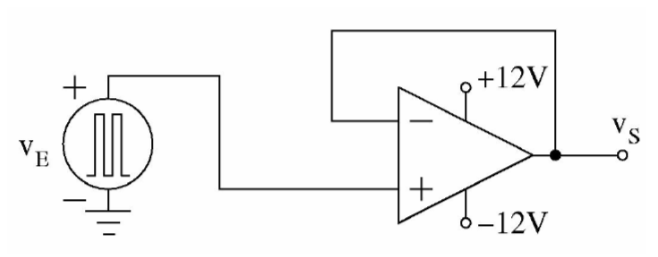
\includegraphics[scale = 0.5]{exp5.png}
  \caption{Medição da faixa de tensão de entrada.}
  \label{fig:circuito6}
\end{figure}

\subsubsection{Parte 1 - Montagem}

O circuito da figura \ref{fig:circuito6} foi montado, obtendo-se a montagem da figura \ref{fig:montagem7}.

\begin{figure}[h]
  \centering
  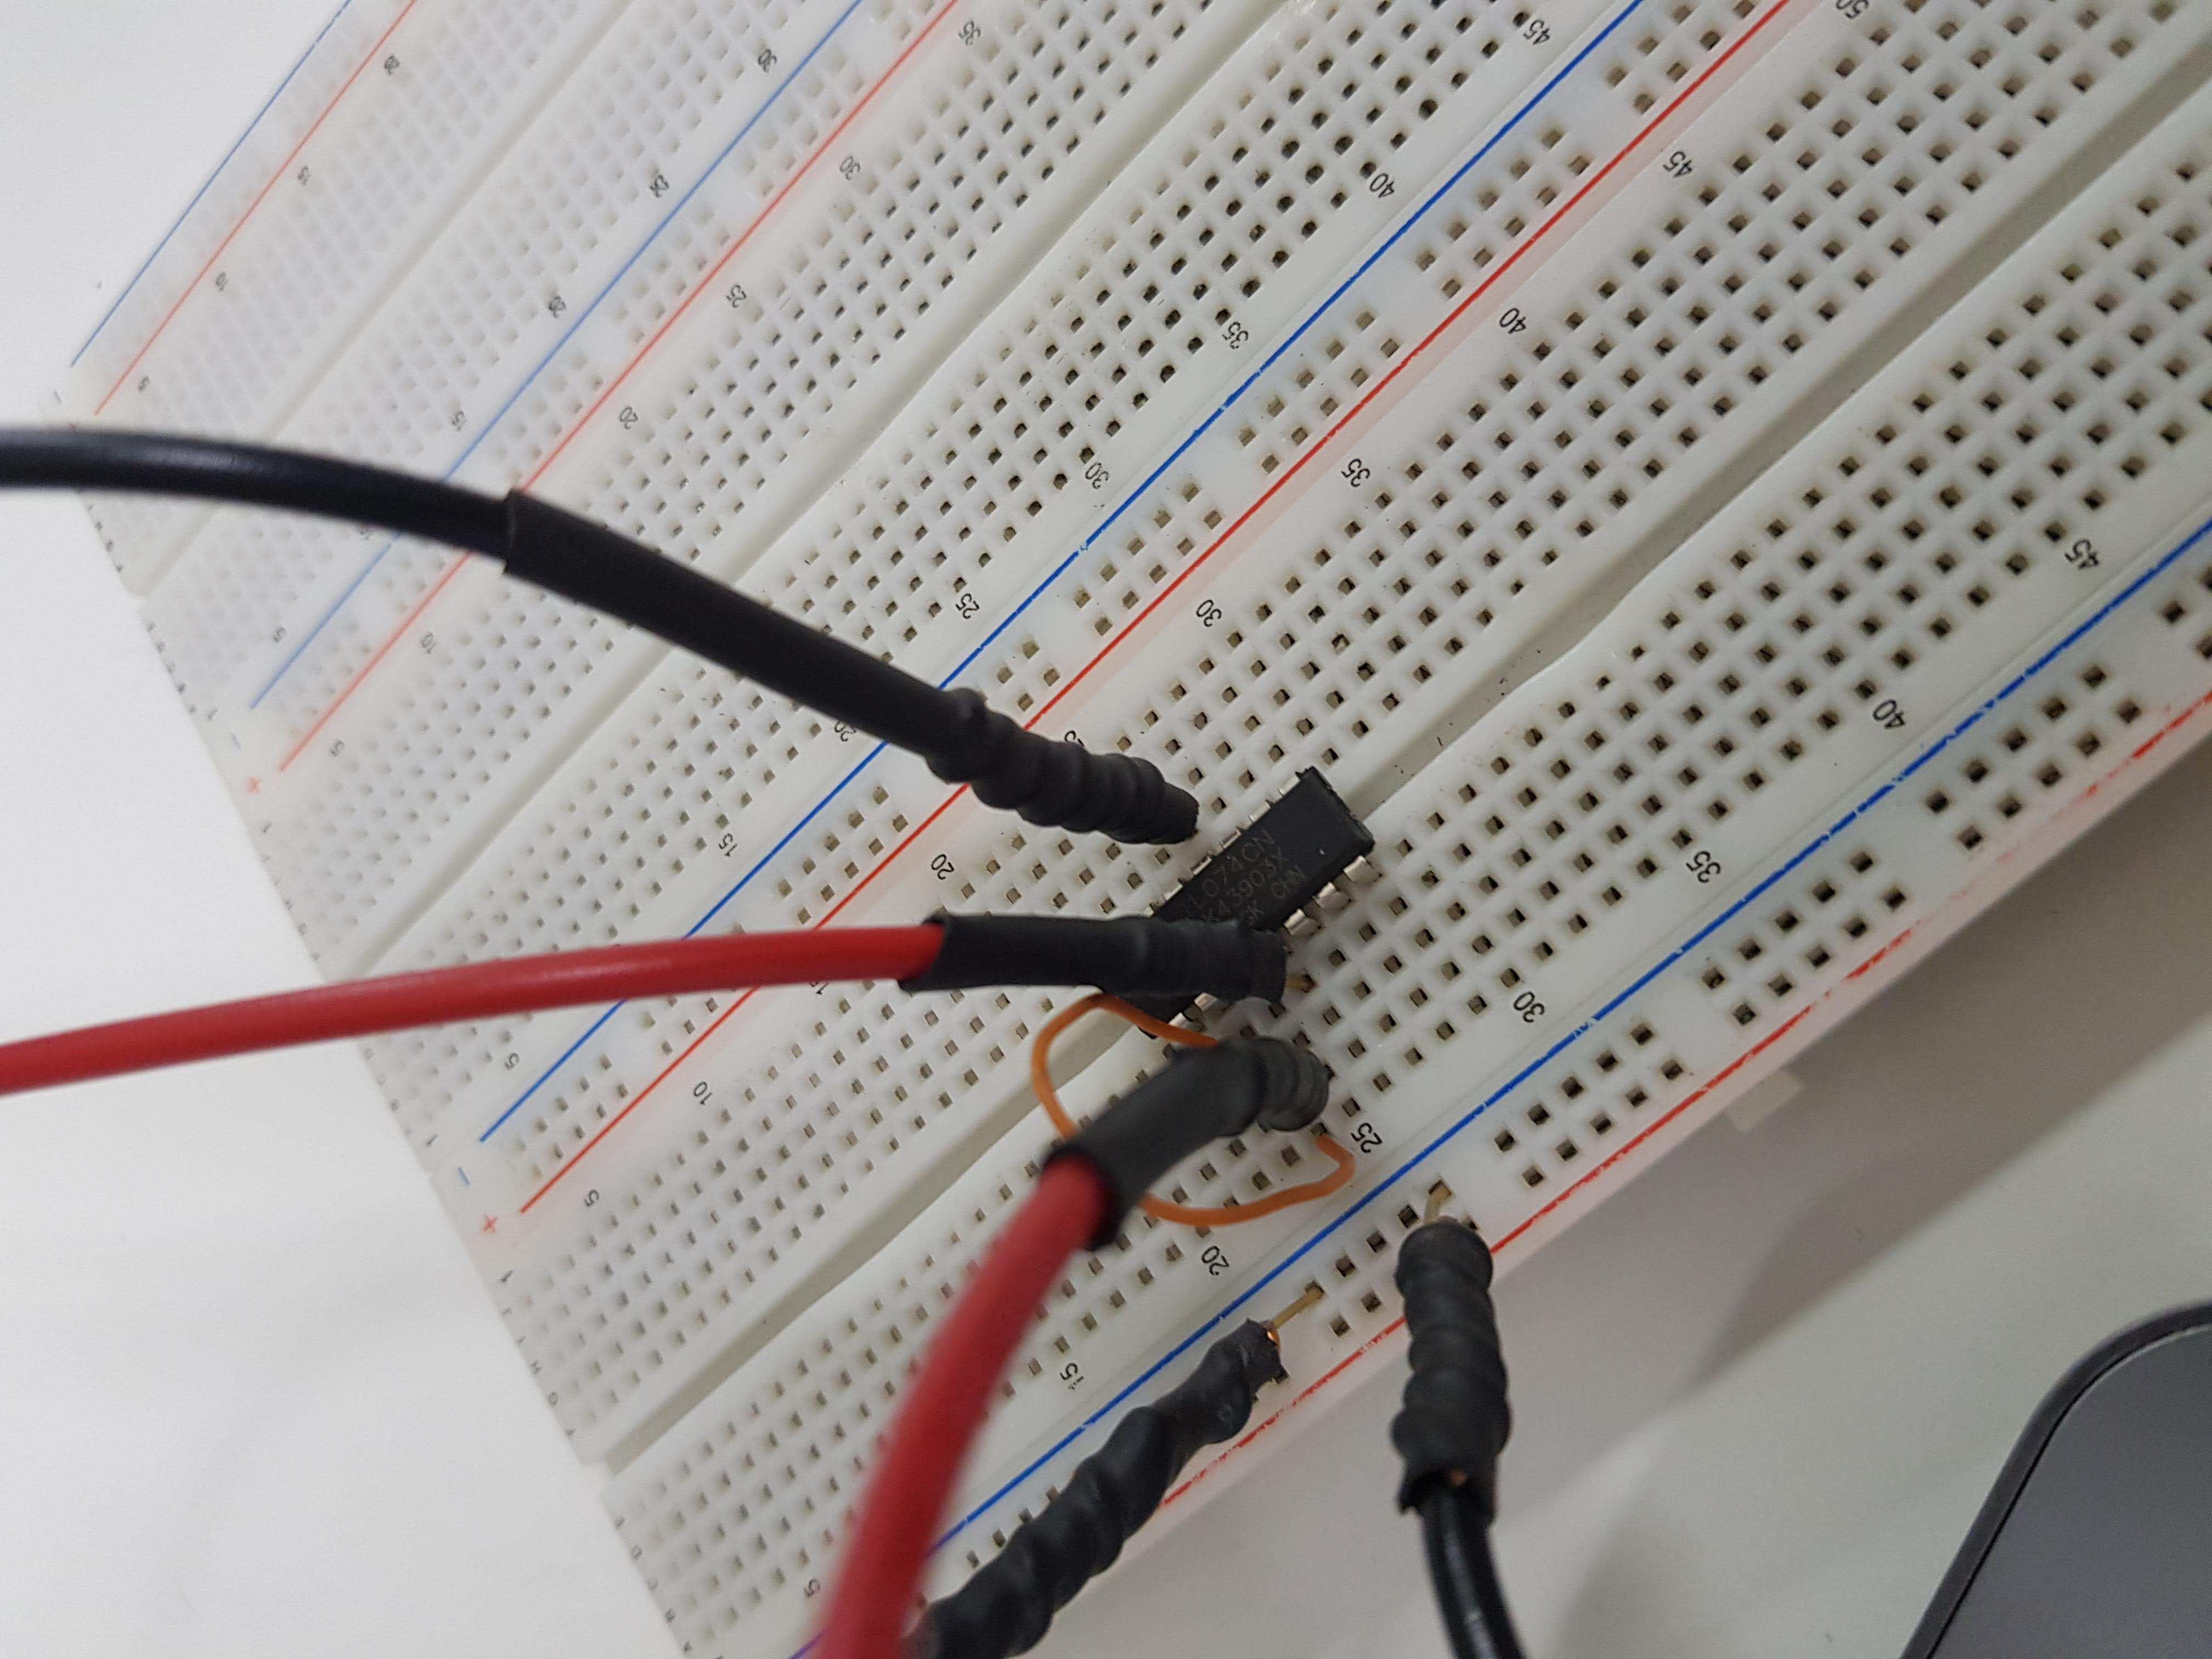
\includegraphics[width = 0.7\textwidth]{circ_5.jpg}
  \caption{Montagem do circuito da figura \ref{fig:circuito6}.}
  \label{fig:montagem7}
\end{figure}

\subsubsection{Parte 2}

Foi colocada na entrada não inversora do amplificador uma onda quadrada de valores máximo e mínimo $1V$ e $-1V$, respectivamente. As tensões de entrada e saída do circuito foram medidas para as segintes frequencias de entrada:
\begin{itemize}
  \item $f_1 = 100$Hz - Figura \ref{fig:inout7}
  \item $f_2 = 1$kHz - Figura \ref{fig:inout8}
  \item $f_3 = 10$kHz - Figura \ref{fig:inout9}
  \item $f_4 = 100$kHz - Figura \ref{fig:inout10}
\end{itemize}

\begin{figure}[h]
  \centering
  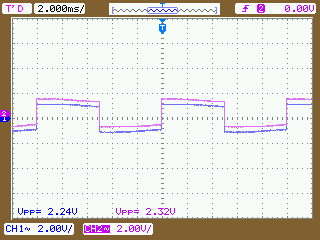
\includegraphics[scale = 0.5]{NewFile7.png}
  \caption{Ondas de entrada e saída para o circuito da figura \ref{fig:circuito6} com frequência de $100$Hz.}
  \label{fig:inout7}
\end{figure}

\begin{figure}[h]
  \centering
  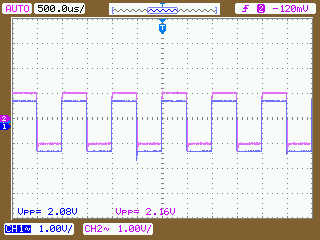
\includegraphics[scale = 0.5]{NewFile8.png}
  \caption{Ondas de entrada e saída para o circuito da figura \ref{fig:circuito6} com frequência de $1$kHz.}
  \label{fig:inout8}
\end{figure}

\begin{figure}[h]
  \centering
  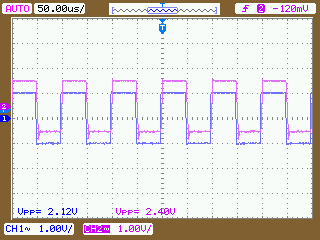
\includegraphics[scale = 0.5]{NewFile9.png}
  \caption{Ondas de entrada e saída para o circuito da figura \ref{fig:circuito6} com frequência de $10$kHz.}
  \label{fig:inout9}
\end{figure}

\begin{figure}[h]
  \centering
  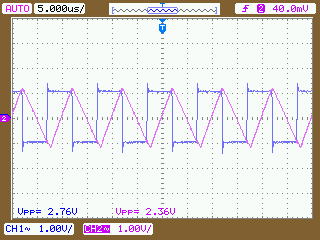
\includegraphics[scale = 0.5]{NewFile10.png}
  \caption{Ondas de entrada e saída para o circuito da figura \ref{fig:circuito6} com frequência de $100$kHz.}
  \label{fig:inout10}
\end{figure}

Para a frequência de $100$kHz pode-se observar o fenômeno do \emph{Slew Rate (SR)}. Foi calculado o SR para a inclinação de subida e de descida pela fórmula

\[{SR} = \frac{\Delta V_O}{\Delta t} V/\mu s\]

De modo que foi obtido o ${SR}_{subida} = 0,55V/\mu s$ e ${SR}_{descida} = 0,42V/\mu s$ que resulta em ${SR}_{médio} = 0,48V/\mu s$ com os valores das figuras \ref{fig:inout11} e \ref{fig:inout12}.

\begin{figure}[h]
  \centering
  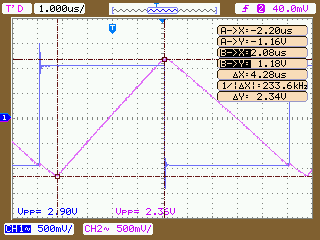
\includegraphics[scale = 0.5]{NewFile11.png}
  \caption{Valores de $\Delta V_O$ ($\Delta Y$) e $\Delta t$($\Delta X$) para a frequencia de $100$kHz.}
  \label{fig:inout11}
\end{figure}

\begin{figure}[h]
  \centering
  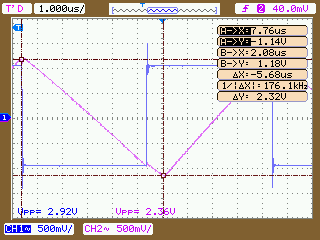
\includegraphics[scale = 0.5]{NewFile12.png}
  \caption{Valores de $\Delta V_O$ ($\Delta Y$) e $\Delta t$($\Delta X$) para a frequencia de $100$kHz.}
  \label{fig:inout12}
\end{figure}

Esse fenômeno se deve ao fato de que o amplificador leva um tempo para atingir a tensão de saída dada uma tensão de entrada, se a tensão varia a uma frequêcia maior do que o tempo necessário para o amplificador atingir a tensão de saída, a forma de onda fica semelhante à da imagem \ref{fig:inout10}.

\chapter{Discussão}

\section{Discussão dos resultados}

Observou-se ao longo do experimento os fenômenos resultantes das imperfeições CC e não-linearidades dos amplificadores operacionais.

Os valores obtidos em geral são próximos dos valores esperados, porém não foram iguais devido ao fato do amplificador não ser ideal. As não linearidades também puderam ser observadas nas formas de ondas obtidas, principalmente nas formas de onda onde ocorre distorção no sinal de saída e através da observação do fenômeno do \emph{Slew Rate}.

\clearpage

\section*{Referências}

[1] SEDRA, Adel S.; SMITH, Kenneth Carless. Microelectronic circuits. New York: Oxford University Press, 1998.

[2] RAZAVI, Behzad; BEHZAD, Razavi. RF microelectronics. New Jersey: Prentice Hall, 1998.

\end{document}
